\chapter{Methodology}

The development of \textbf{Event Blinker} follows an agile, iterative development methodology, progressing through requirements analysis, architecture design, module-wise implementation, integration testing, and deployment.

% Section 3.1 Technology Stack removed as it repeats what was in the Intro/Scope.
\section{Backend Architecture}
The backend (\texttt{server.js}) serves as the central API hub, registering 11 route modules. This modular structure allows each functional area of the application, such as authentication, event management, and ride-sharing, to be managed independently. Each module is equipped with its own set of validation logic and database interactions, which promotes maintainability and scalability. The integration of JSON Web Tokens (JWT) facilitates secure, stateless communication between the server and the various clients, while customized middleware handles cross-origin resource sharing (CORS) and detailed request logging for security audits.

\begin{table}[H]
\centering
\caption{Backend API Route Modules}
\label{tab:api_routes}
\begin{tabular}{@{}llp{7cm}@{}}
\toprule
\textbf{Route Path} & \textbf{Module} & \textbf{Functionality} \\
\midrule
\texttt{/api/auth} & auth.js & User registration and JWT login \\
\texttt{/api/events} & events.js & Event CRUD with PostGIS spatial queries \\
\texttt{/api/likes} & likes.js & Event like/unlike toggle \\
\texttt{/api/checkin} & checkins.js & Event attendance check-in \\
\texttt{/api/chat} & chat.js & Real-time chat with AI bot integration \\
\texttt{/api/rides} & rides.js (925 lines) & Complete ride-sharing lifecycle \\
\texttt{/api/ai} & ai.js & Blinker AI concierge endpoint \\
\texttt{/api/upload} & upload.js & Image upload via Multer \\
\texttt{/api/users} & users.js & User profile management \\
\texttt{/api/organizer} & organizer.js & Organizer-specific event features \\
\texttt{/api/admin} & admin.js (679 lines) & Admin verification workflows \\
\bottomrule
\end{tabular}
\end{table}

% Figure 3.1 (Data Flow) removed.

\section{Geospatial Engine}
Event discovery is powered by PostGIS spatial functions, which extend the PostgreSQL database to support geographic objects. By utilizing the \texttt{GEOMETRY(Point, 4326)} type, we store the precise latitude and longitude coordinates of events and riders. This native support allows the system to perform complex spatial calculations directly within the database engine, ensuring high performance and accuracy even as the dataset grows.

\begin{itemize}[noitemsep]
    \item \texttt{ST\_SetSRID(ST\_Point(lng, lat), 4326)} -- Create spatial points from coordinates.
    \item \texttt{ST\_DWithin(geom, point, radius)} -- Efficiently find events within a given distance.
    \item \texttt{ST\_Distance(geom1, geom2)} -- Calculate the exact distance between geometries for sorting.
    \item \texttt{ST\_AsGeoJSON(geom)} -- Convert geometry objects into GeoJSON for client-side rendering.
\end{itemize}
GiST spatial indexes are meticulously maintained on all location-based fields, \\ such as \texttt{events.location\_geom} and \texttt{riders.current\_location}, ensuring that geospatial queries consistently achieve sub-second response times.

\section{AI Integration (Blinker AI)}
The AI module (\texttt{routes/ai.js}) implements a sophisticated multi-model fallback strategy to guarantee high availability and reliability. By utilizing the OpenRouter API, the application can seamlessly transition between different LLMs, such as LLAMA 3.3 and Gemini Flash, in response to varying API performance or downtime. The integration layer performs dynamic prompt construction, injecting live event data from the database into the LLM context to ensure that the AI's responses are accurate, timely, and culturally localized for the Nepali user base.

\begin{enumerate}[noitemsep]
    \item User sends a message via \texttt{POST /api/ai/chat}.
    \item Backend fetches live event context from PostgreSQL (title, venue, price, time).
    \item A detailed system prompt is constructed with platform knowledge (ride-sharing instructions, ticketing help, Nepali greetings).
    \item The request cycles through 5 LLM models in order: LLAMA 3.3 $\rightarrow$ Gemini Flash $\rightarrow$ Gemini 1.5 $\rightarrow$ LLAMA 3.1 $\rightarrow$ OpenRouter Free.
    \item Each model has a 12-second timeout. If one fails, the next is tried automatically.
\end{enumerate}
\begin{figure}[H]
    \centering
    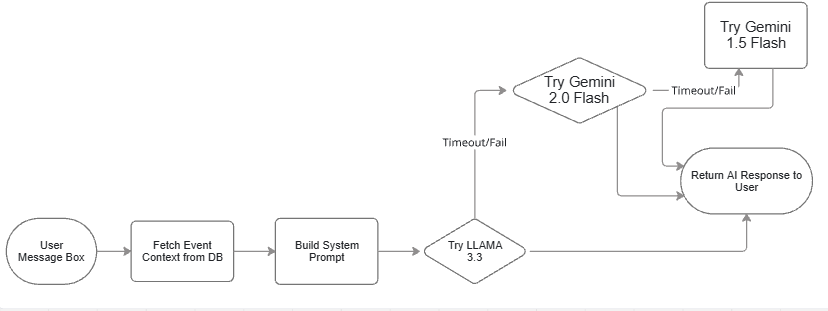
\includegraphics[width=0.8\textwidth]{ai.png}
    \caption{Blinker AI Multi-Model Fallback Strategy}
    \label{fig:ai_flowchart}
\end{figure}

% Figure 3.2 (AI Flowchart) removed.


\section{Ride-Sharing Module}
The ride-sharing system (\texttt{routes/rides.js}, 925 lines) implements a complete lifecycle:

\subsection{Driver Registration (3-Step Process)}
\begin{enumerate}
    \item \textbf{Personal Info} (\texttt{POST /rider/register/personal}): Profile photo, emergency contact, NID, bank details.
    \item \textbf{Vehicle Info} (\texttt{POST /rider/register/vehicle}): Make, model, year, license plate, vehicle type, billbook photo.
    \item \textbf{License Info} (\texttt{POST /rider/register/license}): License number, photo, expiry date, issuing authority.
\end{enumerate}
After all three steps, admin approval is required before the driver can accept rides.

\subsection{Distance Calculation and Pricing}
Distance is computed using the \textbf{Haversine formula} (\texttt{utils/distanceCalculator.js}):

\begin{table}[H]
\centering
\caption{Ride Pricing Model (NPR)}
\label{tab:pricing}
\begin{tabular}{@{}lccc@{}}
\toprule
\textbf{Vehicle Type} & \textbf{Rate/km (NPR)} & \textbf{Base Fare (NPR)} & \textbf{Discount} \\
\midrule
Motorcycle & 15 & 50 & -- \\
Hatchback & 22 & 50 & -- \\
Sedan & 25 & 50 & 5\% ($>$10 km) \\
SUV & 35 & 50 & 10\% ($>$20 km) \\
Van & 40 & 50 & 10\% ($>$20 km) \\
\bottomrule
\end{tabular}
\end{table}

% ---- FIGURE: Ride Lifecycle Flowchart ----
% >>> CREATE THIS: Flowchart showing:
%     Passenger Request → Notify Nearby Riders (Socket.io) → Rider Accepts/Offers Price
%     → Passenger Confirms → Ride In-Progress → Ride Complete → Review
\begin{figure}[H]
    \centering
    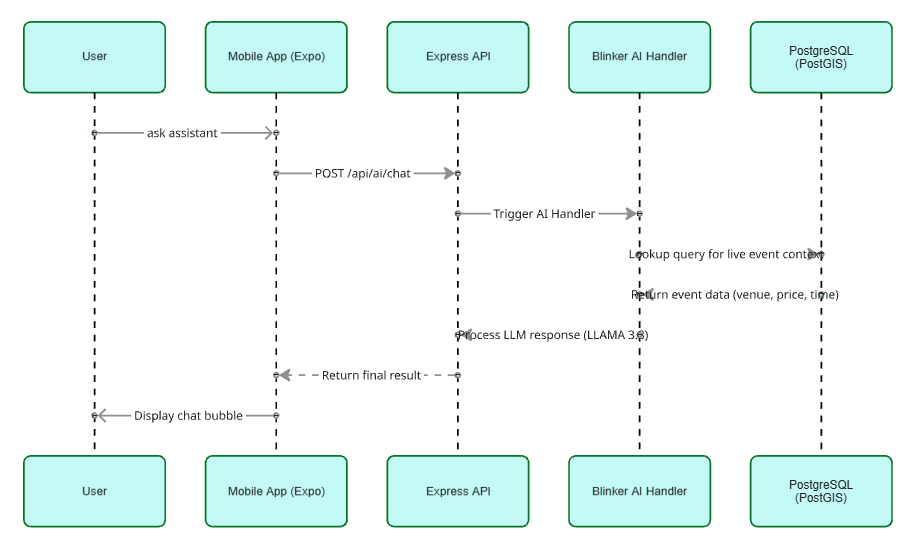
\includegraphics[width=0.8\textwidth]{activity.png}
    \caption{Peer-to-Peer Ride Request Lifecycle}
    \label{fig:ride_lifecycle}
\end{figure}

\section{Real-Time Communication}
Socket.io (\texttt{utils/socket-handler.js}) manages the following real-time events:

\begin{table}[H]
\centering
\caption{Socket.io Events}
\label{tab:socket_events}
\begin{tabular}{@{}lp{8cm}@{}}
\toprule
\textbf{Event} & \textbf{Description} \\
\midrule
\texttt{join:event} / \texttt{leave:event} & User joins/leaves an event chat room \\
\texttt{message:send} / \texttt{message:new} & Send and broadcast chat messages \\
\texttt{event:update-status} & Real-time event status changes \\
\texttt{subscribe:events} & Subscribe to all event updates (map markers) \\
\texttt{ride:new} & Notify nearby riders of a new ride request \\
\texttt{ride:accepted} & Notify passenger that a rider accepted \\
\texttt{ride:started} / \texttt{ride:cancelled} & Ride lifecycle updates \\
\texttt{rider:online} / \texttt{rider:offline} & Driver availability status \\
\bottomrule
\end{tabular}
\end{table}

\section{Mobile Application}
The React Native (Expo) mobile app (\texttt{mobile/}) consists of:

\begin{table}[H]
\centering
\caption{Mobile App Screen Structure}
\label{tab:mobile_screens}
\begin{tabular}{@{}llp{6cm}@{}}
\toprule
\textbf{Screen} & \textbf{File} & \textbf{Functionality} \\
\midrule
Map Discovery & \texttt{(tabs)/map.js} & Mapbox GL with live event markers \\
Events List & \texttt{(tabs)/events.js} & Scrollable event feed \\
Ride Sharing & \texttt{(tabs)/rides.js} (47KB) & Full ride booking/offering UI \\
Live Chat & \texttt{(tabs)/chat.js} (24KB) & Real-time event chat with AI \\
Profile & \texttt{(tabs)/profile.js} & User profile \& settings \\
Event Detail & \texttt{eventDetail.js} & Event info, like, check-in, chat \\
Ride Detail & \texttt{rideDetail.js} (23KB) & Ride tracking \& driver info \\
Ride Map Picker & \texttt{rideMapPicker.js} & Select pickup/dropoff on map \\
Driver Register & \texttt{riderRegister.js} (25KB) & 3-step driver registration form \\
Login/Register & \texttt{auth/login.js}, \texttt{register.js} & Authentication screens \\
\bottomrule
\end{tabular}
\end{table}

State management uses \textbf{Zustand} stores: \texttt{authStore.js}, \texttt{eventStore.js}, and 
\\ \texttt{socketStore.js}.

\section{Web Organizer Portal}
The React/Vite web portal (\texttt{web/src/}) provides organizer tools:
\begin{itemize}[noitemsep]
    \item \texttt{LoginPage.jsx} -- Organizer authentication.
    \item \texttt{DashboardPage.jsx} -- Event overview and metrics.
    \item \texttt{EventsPage.jsx} -- Manage created events.
    \item \texttt{CreateEventPage.jsx} + \texttt{EventForm.jsx} -- Event creation with \texttt{MapPicker.jsx} for location selection.
    \item \texttt{AnalyticsPage.jsx} -- Engagement analytics (likes, check-ins, attendance).
    \item \texttt{ChatManagementPage.jsx} -- View and moderate event chat messages.
    \item \texttt{RiderVerificationPage.jsx} -- Verify rider documents and licenses.
\end{itemize}

\section{Admin Portal}
A standalone HTML admin portal (\texttt{admin-portal/public/index.html}) authenticated via secret token (\texttt{X-Admin-Token}) provides:
\begin{itemize}[noitemsep]
    \item Approve/reject pending organizer registrations.
    \item Approve/reject pending event submissions.
    \item Verify/reject rider registrations (with document review).
    \item Verify/reject driver license submissions.
    \item View all approved events and rider statistics.
\end{itemize}